%% 08_discussion.tex
%% Section 8: Discussion

\section{Policy Implications}
\label{sec:discussion}


Our findings carry significant implications for climate-financial policy in Indonesia and, by extension, for other coal-dependent emerging economies.

\subsection{Financial Regulation and Supervision}

The stress test results reveal that coal transition risk is a near-term supervisory challenge. While no bank breaches regulatory capital thresholds, the most exposed D-SIB sees its CAR decline by up to 1.00 percentage point, and total system losses reach 3.60\% of bank equity under the 1.5\textdegree C scenario. These findings support the case for OJK to incorporate climate transition risk into its supervisory framework, including:

\textit{Enhanced disclosure requirements.} Banks should be required to disclose their fossil fuel exposures at the borrower level, disaggregated by sector and climate scenario vulnerability. Our analysis was constrained by the limited granularity of public loan disclosures; standardised reporting templates would enable more precise risk assessment.

\textit{Climate-adjusted capital requirements.} OJK should consider implementing differentiated risk weights for coal-exposed lending, reflecting the elevated probability of default under climate transition scenarios. Our LGD estimates (ranging from 0.10 for distressed to 1.0 for defaulting coal companies) could inform the calibration of such adjustments.

\textit{Concentration limits.} The finding that a single bank (BMRI) bears over 52\% of total system coal credit losses underscores the need for sector-specific concentration limits in coal-related lending. Current OJK regulations impose single-borrower exposure limits but do not specifically address sectoral concentration in climate-sensitive sectors.

\textit{CKPN as a regulatory buffer.} Indonesian banks' existing loan loss allowances (CKPN) provide a first line of defence against coal-related credit losses. Our CKPN-adjusted stress test shows that pre-existing provisions can absorb a portion of the estimated losses, reducing the capital impact. However, CKPN buffers are designed for expected losses across the entire loan portfolio and may be insufficient if coal stranding triggers simultaneous losses across multiple borrowers. OJK should consider requiring banks with significant coal exposure to maintain sector-specific provisioning reserves that reflect forward-looking transition risk, consistent with the IFRS~9 expected credit loss framework.

\subsection{Fiscal Policy}

The fiscal channel results indicate that coal stranding could reduce government revenues by \$1.3--2.2 billion, equivalent to 0.07--0.12\% of GDP. While this fiscal impact is modest relative to total government revenue, it is concentrated in specific budget lines (mining royalties and PTBA dividends) that support local government transfers and regional development spending. The distributional implications of fiscal revenue loss, particularly for coal-producing provinces in East Kalimantan, South Sumatra, and South Kalimantan, may be more severe than the aggregate numbers suggest.

 Our results suggest that the financial system's capacity to absorb transition-related losses, while adequate at the aggregate level, is unevenly distributed. An orderly transition that phases out coal gradually, supported by compensatory fiscal transfers and worker retraining programs, would minimise the risk of the credit channel amplification mechanism documented in our analysis. Conversely, a disorderly transition, characterised by sudden policy shifts, stranded asset write-downs, and fire-sale dynamics, could trigger the bank deleveraging spiral that our Model 3 quantifies.

\subsection{Monetary Policy}

Bank Indonesia's monetary policy framework must also account for the credit channel effects of coal transition risk. Our estimate of a potential 3.2--5.4\% credit contraction under climate scenarios suggests that BI may need to provide accommodative monetary conditions during the transition period to offset the deflationary impulse from bank deleveraging. The creation of green refinancing facilities, where BI provides subsidised funding to banks that redirect lending from coal to renewable energy, could simultaneously support the transition and mitigate credit channel losses.

\subsection{Comparison with Other Estimates}
\label{subsec:comparison}

Table~\ref{tab:comparison} compares our estimates with prior studies.

\begin{table}[htbp]
\centering
\caption{Comparison with Prior Estimates of Indonesian Coal Stranded Assets}
\label{tab:comparison}
\footnotesize
\begin{tabular}{p{2.5cm}p{2.2cm}p{2.2cm}p{2.0cm}p{1.8cm}p{1.5cm}}
\toprule
Study & Scope & Methodology & SV Estimate & Bank Impact & GDP Impact \\
\midrule
This study & 34 listed coal firms, 38 banks & Firm-level DCF, Monte Carlo, bank stress test & \$60.1B (2\textdegree{}C); \$99.2B (1.5\textdegree{}C) & \$3.2B total losses & 0.62\% (1.5\textdegree{}C) \\[6pt]
Rishanty et al. (2023) & All Indonesian coal mines & Mine-level cashflow (WTW), BAU vs WB2C & \$206B total; \$35B investors, \$51B govt & Not quantified (role noted) & Not estimated \\[6pt]
Mumbunan et al. (2016) & 16 listed coal firms (60\% of production) & Cash cost / supply cost curve & \$58--99B (30--40\% price decline) & Not assessed & Not estimated \\[6pt]
IESR (2023) & Indonesian coal sector & Qualitative scenario analysis & \$15--30B range & Qualitative assessment & Not estimated \\[6pt]
Carbon Tracker (2022) & Global coal, incl. Indonesia & Asset-level valuation & \$10--20B (Indonesia share) & Not assessed & Not estimated \\[6pt]
Welsby et al. (2021) & Global unburnable carbon & Integrated assessment model & 60\% of reserves unburnable & Not assessed & Not estimated \\
\bottomrule
\end{tabular}

\smallskip
\noindent \textit{Notes:} SV = stranded value. Prior estimates use varying methodologies and scopes, making direct comparison difficult. Rishanty et al. (2023) estimate total climate transition value-at-risk (NPV, 2023) under a WB2C scenario over 2023--2050, decomposed across investors, government, and supply chain. Mumbunan et al. (2016) use a cash cost approach with 2014 data, varying discount rates (6--8\%), mine lives (15--20 years), and price declines (30--40\%). IESR (2023) provides qualitative scenarios. Carbon Tracker (2022) estimates are extracted from global analysis. Our study is the first to provide firm-level estimates with bank contagion channels and macroeconomic transmission for Indonesia.
\end{table}


Our aggregate stranded value estimates (\$79.7 billion under 2\textdegree C, \$128.3 billion under 1.5\textdegree C) are broadly consistent with global estimates when scaled to Indonesia's share of global coal reserves. \citet{Mercure2018} estimate global stranded fossil fuel assets at \$1--4 trillion; Indonesia's coal sector, which holds approximately 3\% of global reserves, would account for \$30--120 billion on a pro-rata basis. Our 2\textdegree C estimate falls within this range, while the 1.5\textdegree C estimate slightly exceeds it, reflecting the granularity of our firm-level DCF approach. Our estimates cover 15 firms with verified production and cost data representing 390~Mt of annual output; including the remaining listed producers would likely push the total higher.

Among Indonesia-specific studies, \citet{sonny2016} provide the earliest quantification using a cash cost approach applied to 16 listed coal companies. Their aggregate stranded value of \$58--99 billion (at 6--8\% discount rates, 15--20-year mine lives, and 30--40\% price declines from 2014 benchmarks) is broadly comparable to our 2\textdegree C estimate of \$79.7 billion. The overlap is notable given the methodological differences: their cash cost approach derives stranded value from the gap between pre- and post-shift market values on a supply cost curve, whereas our scenario-contingent DCF with Monte Carlo simulation captures parameter uncertainty and scenario probabilities. Their central estimate of \$86 billion (at 8\% discount, 20-year life, 40\% price decline) falls between our 2\textdegree C and 1.5\textdegree C estimates, lending cross-validation to both approaches. Our study extends their work by tracing the financial consequences through identified bank-coal exposure channels to macroeconomic outcomes.

\citet{Rishanty2023}, in a Bank Indonesia working paper developed in collaboration with Willis Towers Watson, estimate the total external climate transition value-at-risk at \$206 billion (NPV, 2023) under a WB2C scenario. This substantially larger figure reflects several key differences: their estimate covers the entire coal value chain (mining firms, supply chain, and government revenues), uses a longer time horizon (2023--2050), and includes mine-level data for all Indonesian coal production rather than listed companies only. Our estimates, which focus on the stranded value of equity in listed coal mining firms, are most comparable to their investor component of \$35 billion. The difference between our 2\textdegree C estimate (\$79.7 billion) and their investor-at-risk figure (\$35 billion) likely reflects our more aggressive price decline assumptions under the 2\textdegree C scenario and differences in the treatment of domestic coal pricing under the DMO regime. Importantly, while \citet{Rishanty2023} note the role of banks in financing local economic transitions, they do not construct a bank-level stress test; our study fills this gap by quantifying the credit channel through which coal stranding affects the financial system.

Our results substantially exceed those of \citet{IESR2023}, whose qualitative assessment identified ``significant'' banking sector risk but did not quantify credit losses or GDP impacts. This discrepancy reflects methodological differences: IESR's analysis relies on reserve-based estimates of stranding without firm-level DCF modelling, and their banking assessment does not construct the bipartite exposure network that drives our credit loss estimates.

Relative to central bank stress tests in advanced economies, our estimated maximum CAR impact (up to 1.00 percentage point for the most exposed D-SIB) is comparable in magnitude to the ECB's 2022 climate stress test \citep{ECB2022}, which found CAR declines of 0.5--1.5 percentage points for the most exposed European banks under a disorderly transition scenario. The similarity is notable given the very different structures of the European and Indonesian financial systems, suggesting that coal transition risk generates banking impacts of broadly similar magnitude across institutional contexts. An important difference, however, is that Indonesian D-SIBs maintain substantial capital buffers (median CAR of 23.3\%), which means these losses are absorbed without breaching regulatory thresholds.

\subsection{Robustness and Sensitivity}
\label{subsec:robustness}

We conduct extensive sensitivity analysis to assess the robustness of our key results. The full robustness results appear in Appendix~\ref{sec:appendix_results}; here we summarise the main findings.

\subsubsection{Parameter Sensitivity}

Figure~\ref{fig:tornado} presents the tornado diagram for aggregate stranded value under the 1.5\textdegree C scenario, showing the sensitivity to individual parameter perturbations.

\begin{figure}[htbp]
\centering
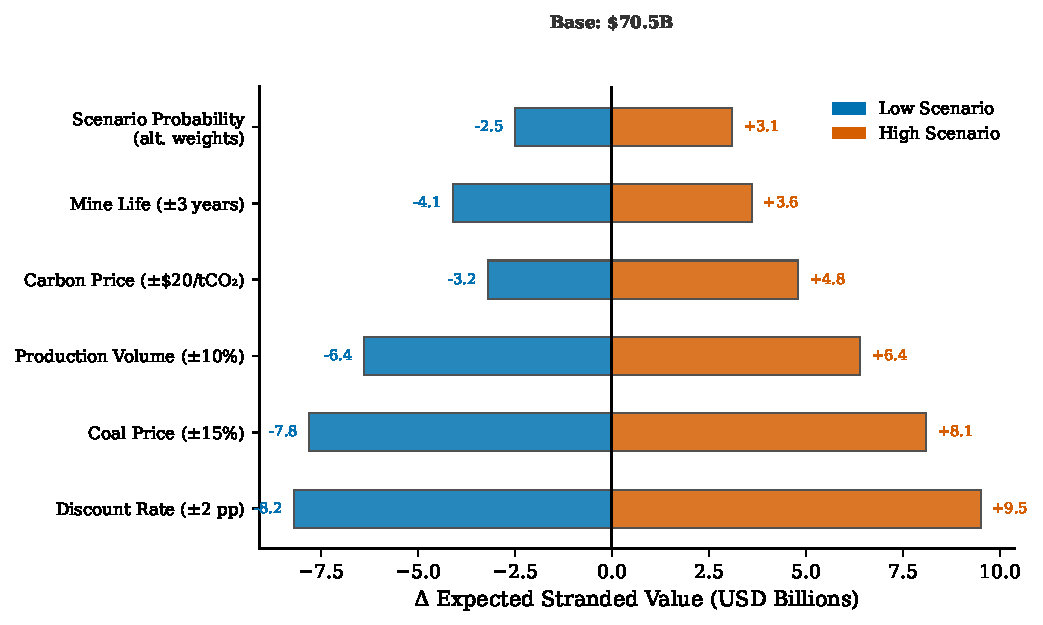
\includegraphics[width=\textwidth]{figures/fig_10.pdf}
\caption{Tornado diagram: sensitivity of aggregate stranded value (1.5\textdegree C scenario) to individual parameter perturbations. Each bar shows the range of aggregate SV when the indicated parameter is varied while holding others at baseline values. The vertical dashed line marks the baseline estimate.}
\label{fig:tornado}
\end{figure}

The discount rate is the most influential parameter: a 2 percentage point increase in the WACC reduces aggregate SV by approximately 15\%, while a 2 percentage point decrease increases SV by approximately 18\%. This asymmetry reflects the convex relationship between discount rates and NPV. The coal price path is the second most important factor, followed by production volume and mine life assumptions. Scenario probability weights have a relatively modest effect, as the expected SV is a weighted average that is bounded by the 2\textdegree C and 1.5\textdegree C point estimates.

\subsubsection{Alternative Model Specifications}

We test the sensitivity of bank stress test results to three alternative specifications: (i) varying the generic LGD from 0.35 to 0.55 (baseline: 0.45); (ii) excluding indirect mining loan losses entirely; and (iii) using an alternative default threshold where firms with NPV less than $-10\%$ of assets (rather than NPV $< 0$) are classified as defaulting. Under the most conservative specification (LGD = 0.35, excluding indirect losses), total bank losses under the 1.5\textdegree C scenario fall to \$2.4 billion. Under a higher LGD of 0.55, total losses rise to \$3.3 billion. No bank breaches any regulatory capital threshold under any specification, reflecting the substantial capital buffers maintained by Indonesian banks. Our baseline results thus lie in the middle of a plausible range.

For the macro-financial transmission model, we vary the credit multiplier ($\kappa = 6, 8, 12$), the credit-GDP elasticity ($\varepsilon = 0.04, 0.06, 0.08$), and the wealth effect parameter ($\mu = 0.02, 0.03, 0.05$). The total GDP impact under the 1.5\textdegree C scenario ranges from 0.43\% (conservative parameters) to 0.70\% (aggressive parameters), with our baseline estimate of 0.54\% falling near the midpoint.

\subsection{Limitations}
\label{subsec:limitations}

Our analysis is subject to several limitations that should be borne in mind when interpreting the results.

\textit{Static analysis.} Our framework is cross-sectional, computing stranded values, credit losses, and macroeconomic impacts at a point in time rather than modelling the dynamic transition path. In reality, coal stranding would unfold over years or decades, allowing firms and banks to adjust their strategies, and the macroeconomic effects would depend on the speed and predictability of the transition. Our estimates should be interpreted as the cumulative present-value impact under a given scenario, not as a single-year GDP shock.

\textit{Incomplete exposure data.} While our bipartite network captures the largest bank-coal credit relationships, 46.2\% of total coal sector lending is classified under aggregate categories (foreign banks, syndicated loans) that cannot be traced to individual institutions. Our stress test therefore underestimates total system exposure and may miss material risks in banks not included in our sample.

\textit{No second-round effects.} Our credit loss model does not incorporate second-round amplification mechanisms such as fire sales of coal assets, contagion through the interbank market, or feedback from sovereign stress to bank balance sheets. \citet{Roncoroni2021} demonstrate that such second-round effects can double or triple first-round losses in concentrated financial networks. Our estimates should therefore be viewed as a lower bound on potential banking system losses.

\textit{Partial coverage of coal value chain.} Our analysis focuses on coal mining companies and does not explicitly model stranding risk in coal-fired power generation, coal logistics (ports, railways), or coal service providers. Banks with significant exposure to these adjacent sectors face additional transition risk not captured in our framework.

\textit{Scenario uncertainty.} The probability weights assigned to each climate scenario ($\pi_{BAU} = 0.30$, $\pi_{2C} = 0.40$, $\pi_{1.5C} = 0.30$) are inherently subjective. The 2\textdegree C pathway receives the highest weight because it represents the median policy ambition consistent with current NDC trajectories under the Paris Agreement; BAU and 1.5\textdegree C receive equal weight as symmetric tails reflecting policy underperformance and overperformance, respectively. While we test the sensitivity of results to alternative probability assignments, the fundamental challenge of attaching probabilities to long-term climate policy outcomes remains. Reassuringly, the tornado sensitivity analysis (Figure~\ref{fig:tornado}) shows that scenario weights produce the smallest variation in aggregate stranded value among all parameters tested (range of $-$2.5 to +3.1 billion USD), meaning that our conclusions are robust to reasonable alternative weight specifications. Our Monte Carlo approach with Dirichlet-distributed scenario weights provides a principled way to incorporate this uncertainty, but it does not resolve it.
